\documentclass[a4paper, 12pt]{article}

\usepackage{graphicx}
\graphicspath{ {../Images/} }
\usepackage[utf8]{inputenc}
\usepackage[T1]{fontenc}
\usepackage{textcomp}
\usepackage{amssymb}
\usepackage{newtxtext} \usepackage{newtxmath}
\usepackage{amsmath, amssymb}
\newtheorem{problem}{Problem}
\newtheorem{example}{Example}
\newtheorem{lemma}{Lemma}
\newtheorem{theorem}{Theorem}
\newtheorem{problem}{Problem}
\newtheorem{example}{Example} \newtheorem{definition}{Definition}
\newtheorem{lemma}{Lemma}
\newtheorem{theorem}{Theorem}


\begin{document}

    

\pagebreak

\section{Clase 1}

\subsection{Info de la materia}

\textit{Mail del profesor.} daniel.penazzi@unc.edu.ar

\textit{Temas a ver.}

\begin{itemize}
    \item Coloreo de grafos 
    \item Flujos en network 
    \item Matchings 
    \item Códigos de correción de errores
    \item P-NP (Complejidad computacional)
    \item Inteligencia artifical
\end{itemize}

La materia tiene tres partes: teórico, práctico y proyecto de programación. Solo
la parte práctica tiene promoción (se explica abajo). El final tiene parte
teórica y parte práctica. La parte teórica es demostrar uno de tres teoremas
dados a priori. La parte práctica tiene ejercicios de demostración o pensamiento
y de resolución de problemas.

La parte práctica se promociona si se aprueban los dos parciales, con cualquer
nota $\geq 4$. De promocionarlo, la parte práctica del final no es necesaria.

El proyecto de programación tiene dos partes. La primera es leer un grafo y
cargar los datos al programa. La segunda es un problema de coloreo de grafos. La
fecha de entrega de la parte uno es en dos o tres semanas a partir de hoy
(13/03). La parte importante es la parte 2.

La biliografía está en el programa 2023.

\subsection{Grafos}

\begin{definition}
    Una grafo es una $2$-upla $G = (V, E)$ con $V$ un conjunto cualquiera (finito) y $E
    \subseteq \left\{ A \subseteq V : |A| = 2 \right\} $
\end{definition}


\small
\begin{quote}

\textbf{Nota.} La restricción de finitud es sólo de esta materia. 

\end{quote}
\normalsize

\begin{center}
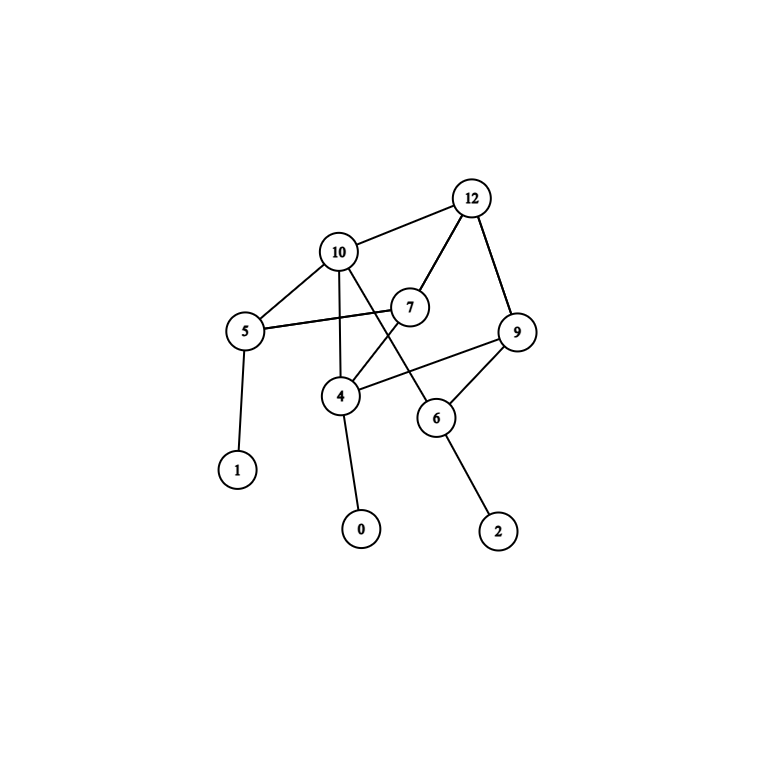
\includegraphics[scale=0.3]{graph}
\end{center}

Los elementos de $V$ se llaman vértices o nodos. Los elementos de $E$ se llaman
lados o aristas. Por convención, a menos que digamos lo contrario, es que $|V| =
n$ y $|E| = m$.

\begin{definition}
    Un camino en un grafo $G = (V, E) $ es una sucesión de vértices $v_1,
    \ldots, v_r$, con $ v_i \in V$ para todo $i$, tal que $\left\{ v_j, v_{j+1}
    \right\} \in E $ para todo $1 \leq j < r$. 
\end{definition}


Dado un camino $v_1, \ldots, v_r$, si $v_1 = x, v_r = y$, decimos que es un
camino de $x$ a $y$. Para todo $G = (V, E)$ definimos la relación binaria 

$$\sim ~:=\left\{ (x, y) \in V^2 : \text{ existe un camino de $x$ a $y$ }  \right\} $$

Es decir, $x \sim y$ denota la relación de que existe un camino entre $x$ e $y$.
Es trivial comproabar que $\sim$ es una relación de equivalencia. Cada clase de
equivalencia $a / \sim$ con $a \in V$ se llama una componente conexa de $G$.

\begin{definition}
    Decimos que $G$ es conexo si y solo si tiene una sola componente conexa. Es
    decir, si $|V \sim ~ | = 1$.
\end{definition}


\small
\begin{quote}

El profesor no mencionó esto pero es lindo recordar (si alguien ha cursado
lógica) que el conjunto de clases de equivalencia $A / R$ de un conjunto a sobre
una relación binaria $R$ puede en sí mismo darse como un grupo de grafos
disconexos. Por ejemplo, abajo se dan los grafos de un espacio cociente con
siete clases de equivalencia; cada par de vértices unidos por un lado
corresponde a dos elementos equivalentes.


\begin{center}
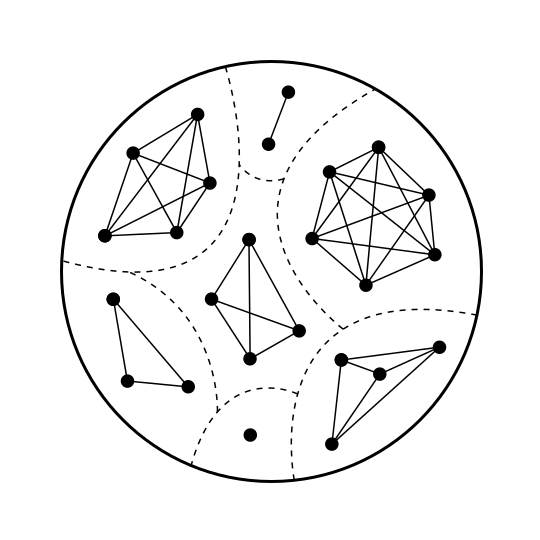
\includegraphics[scale=0.25]{equiv}
\end{center}

Fíjense que de esto se sigue un dato curioso (aunque tal vez irrelevante): Si
$G = (V, E) $ es un grafo conexo con $n$ vértices, el grafo que describe la clase de
equivalencia de $V$ es $K_n$.

\end{quote}
\normalsize

\begin{definition}
    Decimos que un grafo $H = (W, F)$ es un subgrafo de $G =(V, E)$ si
    $W \subseteq V, F \subseteq E$.
\end{definition}

A veces usamos $H \subseteq G$ para decir "$H$ es un subgrafo de $G$", pero no
debe entenderse por esto que $H$ y $G$ son conjuntos.

Observe que no todo $W \subseteq V, F \subseteq E$ satisfacen que $(W, F)$ es un
grafo. Por ejemplo ejemplo, si $F = \emptyset$ tenemos $F \subseteq E$, pero $F$
no cumple la propiedad de que todos sus elementos sean conjuntos con cardinalidad $2$.


\textbf{Convención}. Escribimos $xy$ para denotar $\left\{ x, y \right\} $.

\textbf{Convención}. Si bien cualquier elemento puede ser un vértice, usualmente
dado un grafo $G(V, E) $ asumimos que $V = \left\{ 0, 1, \ldots, n-1 \right\} $. 

\begin{definition}[Densidad]
    Decimos que un grafo es denso si $m = O(n^2)$. Decimos que un grafo es raro
    si $m = O(n)$.
\end{definition}


\small
\begin{quote}

\textbf{Random fact}. Recuerde que "raro" no sólo significa "inusual" sino que es el
antónimo de "denso". La etimología inglesa es más interesante:
La palabra \textit{Weird} (raro) significaba, en la edad media, destino. Por
eso, en la balada medieval \textit{True Thomas}, se lee "Weird shall never
daunton me": El destino nunca ha de asustarme. Se debe a una antigua leyenda
nórdica en la cual las \textit{Weird sisters}, diosas terribles, tejían el
destino de los hombres. Si le da curiosidad:

https://en.wikipedia.org/wiki/Three_Witches

\end{quote}
\normalsize

\begin{definition}
    Dado $G = (V, E) $, si $x \in V$, $\Gamma(x) := \left\{ y \in V : \left\{ x,
        y\right\}  \in E
\right\} $ se llama el vecindario de $x$. 
\end{definition}

Si $y \in \Gamma(x)$, decimos que $y$
es un vecino de $x$.  El grado de $x$, denotado $d(x)$, es la cantidad de
vecinos de $x$; es decir, $d(x) = |\Gamma(x)|$.
Usamos $\delta = \min \left\{ d(x) : x \in V \right\} $ y $\Delta = \max \left\{
d(x) : x \in V\right\} $. Si $\delta = \Delta$ se dice que $G$ es regular. Por
ejemplo, los
grafos cíclicos y los completos son regulares.



\subsection{Repaso de BFS y DFS}

\textit{A completar.}






\subsection{Los grafos $K_n$ y $C_n$}
\label{famosos}

\begin{itemize}
    \item $K_n$ : El grafo completo en $n$ vértices se define 

        $$K_n = \left( \left\{
        1, 2, \ldots, n\right\}, \left\{ \left\{ x, y \right\}  : x, y \in \left\{ 1, 2, \ldots, n
    \right\}  \right\}   \right) $$

    Es el grafo de $n$ elementos donde todos los vértices están conectados unos
    con otros. Resulta que que $m = \binom{n}{2}$. Lo cual implica que $m =
    O(n^2)$.

    \item  $C_n$: El grafo cíclico 

        $$C_n = \left( \left{ 1, 2, \ldots, n \right},
        \left\{ 12, 23, 34, \ldots, (n-1)n, n1 \right\}   \right)$$

        Una observación es
        que $C_3 = K_3$; pero de allí en adelante difieren.
\end{itemize}




\subsection{Coloreo de grafos}

\begin{definition}
    Un coloreo propio de $G = (V, E) $ con $k$ colores es una función  

    \begin{align*}
        C : V \mapsto A
    \end{align*}

    con $|A| = k$ y tal que $xy \in A\Rightarrow C(x) \neq C(y)$.
\end{definition}

Intuitivamente, un coloreo asigna $k$ propiedades a los vértices de modo tal que
ningún par de grafos adyacentes cumple la misma propiedad. 


\small
\begin{quote}

\textbf{Nota.} Hace unos meses escrbí un algoritmo de coloreo en C. Es el
segundo algoritmo dado en esta entrada: 

https://slopezpereyra.github.io/2023-10-29-Hamiltonian/

No prometo que sea muy prolijo o esté bien explicado; ya en general uno es tonto
y encima de tonto no sabe de grafos. Pero tal vez a alguien le sirva, qué se yo.

\end{quote}
\normalsize


\begin{definition}
    El número cromático de un grafo $G= (V, E) $ es 

    \begin{align*}
        \chi(G) = \min_k \left( \exists \text{ coloreo propio de $G$ con $k$
        colores} \right) 
    \end{align*}
\end{definition}

No se conoce un algoritmo polinomial que calcule $\chi(G)$. El proyecto será dar
un algoritmo polinomial que se aproxime a $\chi$.

\subsection{Un algoritmo greedy de coloreo}
~ ~ 

El algoritmo colorea un grafo $G$ con vértices $v_1, \ldots, v_n$ y colores $\left\{
c_1, c_2, \ldots, c_n \right\} $. Para que el algoritmo funcione, los colores
deben tener un orden; por eso se usan números para denotarlos. También se
requiere que los vértices tengan un orden (en este caso dado por los
subíndices).


\small
\begin{quote}

\textbf{Invariante del algoritmo.} Los coloreos parciales son propios. Es decir,
a medida que se va coloreando iterativamente el grafo, en cada paso el coloreo
resultante debe ser propio.

\textbf{Pasos del algoritmo}. 

\textit{(1)} $C(v_1) = c_1$.

\textit{(2)} $C(v_k) = $ mínimo color que mantenga un coloreo propio (que
satisfaga el invariante).

\end{quote}
\normalsize



\subsection{Acotando $\chi$}

Generalmente nos interesa encontar $\chi(G)$ dado un grafo $G = (V, E) $. Damos
unas pautas y observaciones generales para acotar $\chi(G)$ y así facilitar su
hallazgo.

\begin{lemma}[(El profesor no dio esto como un lema pero yo sí)]
    Si existe un coloreo propio de $G = (V, E)$ con $k$ colores, entonces
    $\chi(G) \leq k$.
\end{lemma}


\small
\begin{quote}

\textbf{Proof.} Es trivial por definición de $\chi$ ($\chi$ es el mínimo $k$ en
el conjunto de los coloreos posibles de $G$ con $k$ colores).

\end{quote}
\normalsize

El lema significa que para acotar $\chi$ por arriba solo basta dar un coloreo
con $k$ colores.

\begin{lemma}
    Si $H$ es un subrafo de $G$, $\chi(H) \leq \chi(G)$.
\end{lemma}

Este lema nos dice que podemos acotar $\chi$ por abajo si encontramos un
subgrafo de $G$ cuyo número cromático es conocido. Es fácil ver que $\chi(K_r) =
r$ para todo $r > 1$. Es menos directo pero en clase se demostró que

\begin{align*}
    \chi(C_r) = \begin{cases}
        2 & r \mod 2 \equiv 0 \\ 
        3 & r \mod 2 \equiv 1
    \end{cases}
\end{align*}

Esto, en combinación con el último lema, nos dice que podemos acotar $\chi(G)$
por abajo simplemente observando si $G$ contiene algún $C_r$  o $K_r$ como
subgrafo. En el caso $C_r$, la cota inferior dada en el caso par, con $\chi(C_r)
= 2$, es trivial (todo grafo necesita al menos dos colores). Por eso nos
quedamos con el siguiente teorema: 

\begin{theorem}
    Sea $G = (V, E) $ un grafo. Si $C_r \subseteq G$ con $r$ impar entonces
    $\chi(G) \geq 3$. Si $K_r \subseteq G$ entonces $\chi(G) \geq r$.
\end{theorem}

\begin{theorem}
    Si $\chi(G) \geq 3$, entonces $G$ contiene un ciclo impar.
\end{theorem}


\small
\begin{quote}

\textbf{Proof.} Damos una prueba algorítmica. Llamamos a a este algoritmo
"bipartito" o "2-color". En tiempo polinomial, determina si $G$ se puede
colorear con dos colores; si $\chi(G) = 2$ da un coloreo, de otro modo devuelve
un ciclo impar que es subgrafo de $G$. (El profe no llegó a dar la prueba.)

\end{quote}
\normalsize








\end{document}



